% ============================================================================
% Chapter 7: Experimental Results & Discussion
% (formerly Chapter 9)
% ============================================================================

\chapter{Experimental Results and Discussion}
\label{chap:results}

This chapter presents the experimental methodology, test results, and comprehensive analysis for the AUSRA system across mechanical, electrical, sensor integration, and autonomous navigation subsystems. The results validate the design decisions made throughout the project and demonstrate the system's readiness for collaborative 2D mapping applications.

\section{Mechanical Testing and Validation}
\label{sec:mechanical_testing}

\subsection{Structural Analysis Results}

The mechanical prototype underwent rigorous Finite Element Analysis (FEA) in SolidWorks to validate structural integrity under operational loads. Two plate thickness configurations (3mm and 6mm aluminum) were analyzed to determine the optimal balance between weight and strength.

\subsubsection{Von Mises Stress Analysis}

The stress analysis revealed that both configurations remain well within the material's yield strength under maximum loading conditions.

\begin{table}[H]
\centering
\caption{Von Mises Stress Analysis Results}
\label{tab:stress_results}
\begin{tabular}{|l|c|c|c|c|}
\hline
\textbf{Configuration} & \textbf{Max Stress} & \textbf{Yield Strength} & \textbf{Safety Factor} & \textbf{Status} \\
\hline
3mm Plate & 2.89 MPa & 275 MPa & 95.16 & Pass \\
6mm Plate & 1.45 MPa & 275 MPa & 189.66 & Pass \\
Full Assembly & 8.72 MPa & 275 MPa & 31.54 & Pass \\
\hline
\end{tabular}
\end{table}

\subsubsection{Displacement Analysis}

Maximum displacement under 5 kg payload conditions was measured at critical mounting points.

\begin{table}[H]
\centering
\caption{Displacement Analysis Results}
\label{tab:displacement_results}
\begin{tabular}{|l|c|c|c|}
\hline
\textbf{Configuration} & \textbf{Max Displacement} & \textbf{Allowable} & \textbf{Status} \\
\hline
3mm Plate & 0.089 mm & 2.0 mm & Pass \\
6mm Plate & 0.011 mm & 2.0 mm & Pass \\
Full Assembly & 0.156 mm & 2.0 mm & Pass \\
\hline
\end{tabular}
\end{table}

\subsubsection{Design Decision}

Based on the FEA results, the 3mm plate configuration was selected for the final design. While both configurations exceed safety requirements by a significant margin, the 3mm plate offers:
\begin{itemize}
    \item \textbf{Weight Reduction:} Approximately 50\% lighter than the 6mm configuration
    \item \textbf{Adequate Safety Factor:} Minimum safety factor of 31.54 exceeds the required factor of 2.0
    \item \textbf{Cost Efficiency:} Reduced material cost per robot unit
    \item \textbf{Swarm Scalability:} Lower weight enables longer battery life for extended mapping missions
\end{itemize}

\subsection{Operational Testing Results}

\begin{table}[H]
\centering
\caption{Mechanical Operational Test Results}
\label{tab:mech_operational}
\begin{tabular}{|l|c|c|c|}
\hline
\textbf{Test Parameter} & \textbf{Target} & \textbf{Measured} & \textbf{Status} \\
\hline
Payload Capacity & 5.0 kg & 5.2 kg & Pass \\
Total Robot Weight & $<$ 3.0 kg & 2.4 kg & Pass \\
Ground Clearance & 15 mm & 18 mm & Pass \\
Maximum Speed & 0.5 m/s & 0.52 m/s & Pass \\
Rotation Speed & 1.0 rad/s & 1.2 rad/s & Pass \\
\hline
\end{tabular}
\end{table}

% ============================================================================
\section{Electrical System Validation}
\label{sec:electrical_testing}

\subsection{Power System Performance}

The dual-rail power architecture was tested for voltage stability, current capacity, and runtime under various load conditions.

\begin{table}[H]
\centering
\caption{Power System Test Results}
\label{tab:power_test_results}
\begin{tabular}{|l|c|c|c|}
\hline
\textbf{Parameter} & \textbf{Expected} & \textbf{Measured} & \textbf{Deviation} \\
\hline
Battery Capacity & 5000 mAh & 4850 mAh & -3.0\% \\
12V Rail (No Load) & 12.0 V & 12.1 V & +0.8\% \\
12V Rail (Full Load) & 11.5 V & 11.7 V & +1.7\% \\
5V Rail & 5.0 V & 5.02 V & +0.4\% \\
3.3V Rail & 3.3 V & 3.31 V & +0.3\% \\
Peak Current Draw & 8.0 A & 7.2 A & -10\% \\
Idle Current Draw & 1.5 A & 1.3 A & -13\% \\
Battery Runtime (Idle) & 3.2 hrs & 3.7 hrs & +15.6\% \\
Battery Runtime (Active) & 1.5 hrs & 1.8 hrs & +20\% \\
\hline
\end{tabular}
\end{table}

\subsection{Motor Control Performance}

The Cytron MDD3A dual-channel motor drivers were validated for PWM response and current handling.

\begin{table}[H]
\centering
\caption{Motor Driver Performance Results}
\label{tab:motor_driver_results}
\begin{tabular}{|l|c|c|}
\hline
\textbf{Parameter} & \textbf{Specification} & \textbf{Measured} \\
\hline
PWM Frequency & 20 kHz & 20 kHz \\
PWM Resolution & 8-bit (256 levels) & 256 levels \\
Peak Current per Channel & 3.0 A & 2.8 A \\
Continuous Current & 1.5 A & 1.2 A \\
Response Time & $<$ 10 ms & 8 ms \\
\hline
\end{tabular}
\end{table}

\subsection{Microcontroller Selection Validation}

The ESP32-S3 was selected through a weighted selection matrix comparing three candidates for the low-level control unit.

\begin{table}[H]
\centering
\caption{Microcontroller Selection Matrix Results}
\label{tab:mcu_selection_results}
\begin{tabular}{|l|c|c|c|c|}
\hline
\textbf{Criteria} & \textbf{Weight} & \textbf{Teensy 4.1} & \textbf{STM32F411} & \textbf{ESP32-S3} \\
\hline
Real-Time Performance & 5 & 25 & 20 & 20 \\
micro-ROS Compatibility & 5 & 20 & 15 & 25 \\
Peripheral Count & 4 & 20 & 16 & 16 \\
Power Consumption & 3 & 9 & 12 & 12 \\
Development Ecosystem & 4 & 16 & 12 & 20 \\
Cost & 3 & 6 & 12 & 15 \\
\hline
\textbf{Total Score} & & \textbf{96} & \textbf{87} & \textbf{108} \\
\hline
\end{tabular}
\end{table}

The ESP32-S3 achieved the highest score (108 points), primarily due to its native micro-ROS support and excellent development ecosystem, making it the optimal choice for seamless ROS 2 integration.

% ============================================================================
\section{IMU Integration and Sensor Fusion Results}
\label{sec:imu_results}

\subsection{IMU Hardware Selection}

The MPU-9250 was selected through comprehensive evaluation of IMU configurations and specific models.

\subsubsection{IMU Configuration Comparison}

\begin{table}[H]
\centering
\caption{IMU Configuration Selection Matrix}
\label{tab:imu_config_selection}
\begin{tabular}{|l|c|c|c|c|c|c|c|}
\hline
 & & \multicolumn{2}{c|}{\textbf{6-Axis}} & \multicolumn{2}{c|}{\textbf{9-Axis}} & \multicolumn{2}{c|}{\textbf{Fusion}} \\
\textbf{Criteria} & \textbf{Wt.} & \textbf{R} & \textbf{WS} & \textbf{R} & \textbf{WS} & \textbf{R} & \textbf{WS} \\
\hline
Accuracy \& Performance & 5 & 4 & 20 & 4 & 20 & 5 & 25 \\
Cost & 4 & 5 & 20 & 4 & 16 & 2 & 8 \\
Software Ecosystem & 4 & 4 & 16 & 5 & 20 & 4 & 16 \\
Size \& Weight & 3 & 5 & 15 & 5 & 15 & 3 & 9 \\
Power Consumption & 3 & 5 & 15 & 4 & 12 & 3 & 9 \\
Magnetometer Benefit & 2 & 1 & 2 & 5 & 10 & 5 & 10 \\
\hline
\textbf{Final Score} & & \multicolumn{2}{c|}{\textbf{88}} & \multicolumn{2}{c|}{\textbf{93}} & \multicolumn{2}{c|}{\textbf{67}} \\
\hline
\end{tabular}
\end{table}

\subsubsection{IMU Model Comparison}

\begin{table}[H]
\centering
\caption{IMU Model Selection Matrix}
\label{tab:imu_model_selection}
\begin{tabular}{|l|c|c|c|c|c|c|c|}
\hline
 & & \multicolumn{2}{c|}{\textbf{MPU-9250}} & \multicolumn{2}{c|}{\textbf{BNO055}} & \multicolumn{2}{c|}{\textbf{ICM-20948}} \\
\textbf{Criteria} & \textbf{Wt.} & \textbf{R} & \textbf{WS} & \textbf{R} & \textbf{WS} & \textbf{R} & \textbf{WS} \\
\hline
Sensor Performance & 5 & 4 & 20 & 5 & 25 & 5 & 25 \\
Cost-Effectiveness & 4 & 5 & 20 & 2 & 8 & 3 & 12 \\
Size \& Weight & 3 & 4 & 12 & 3 & 9 & 4 & 12 \\
Software Ecosystem & 4 & 5 & 20 & 4 & 16 & 3 & 12 \\
Power Consumption & 3 & 4 & 12 & 4 & 12 & 4 & 12 \\
Availability & 3 & 5 & 15 & 2 & 6 & 1 & 3 \\
\hline
\textbf{Final Score} & & \multicolumn{2}{c|}{\textbf{99}} & \multicolumn{2}{c|}{\textbf{76}} & \multicolumn{2}{c|}{\textbf{76}} \\
\hline
\end{tabular}
\end{table}

The MPU-9250 achieved the highest score (99 points) due to its extensive software ecosystem, cost-effectiveness (\$15-20 vs \$35-45 for BNO055), and excellent availability---critical factors for swarm deployment where sensor costs must be managed across multiple robots.

\subsection{IMU Calibration Results}

Calibration procedures were validated through statistical analysis of 10,000 samples with the sensor stationary.

\begin{table}[H]
\centering
\caption{IMU Calibration and Noise Characterization}
\label{tab:imu_calibration}
\begin{tabular}{|l|c|c|c|}
\hline
\textbf{Parameter} & \textbf{Specification} & \textbf{Measured} & \textbf{Status} \\
\hline
Accelerometer Noise (X,Y) & $<$ 0.1 m/s$^2$ & 0.05 m/s$^2$ & Pass \\
Accelerometer Noise (Z) & $<$ 0.1 m/s$^2$ & 0.05 m/s$^2$ & Pass \\
Gravity Measurement & 9.81 m/s$^2$ & 9.81 m/s$^2$ & Pass \\
Gyroscope Noise & $<$ 0.05 rad/s & 0.01--0.02 rad/s & Pass \\
Gyroscope Bias Drift & $<$ 0.2°/s & $<$ 0.1°/s & Pass \\
Magnetometer Field & $\sim$45 $\mu$T & 45 $\mu$T & Pass \\
\hline
\end{tabular}
\end{table}

\subsection{Extended Kalman Filter Performance}

The robot\_localization EKF was configured and tuned for optimal sensor fusion performance.

\begin{table}[H]
\centering
\caption{EKF Performance Metrics}
\label{tab:ekf_performance}
\begin{tabular}{|l|c|c|}
\hline
\textbf{Metric} & \textbf{Target} & \textbf{Achieved} \\
\hline
Orientation Accuracy (Yaw) & $<$ 3° RMS & 2° RMS \\
Orientation Accuracy (Pitch/Roll) & $<$ 2° RMS & 1.5° RMS \\
Settling Time (95\% convergence) & $<$ 1.0 s & 0.5 s \\
Heading Drift (IMU only) & --- & 1°/minute \\
Update Rate & 50 Hz & 50 Hz \\
\hline
\end{tabular}
\end{table}

\subsection{System Latency Comparison}

The transition from ESP32 bridge to direct Jetson Orin Nano integration demonstrated significant latency improvements.

\begin{table}[H]
\centering
\caption{IMU System Latency Analysis}
\label{tab:imu_latency}
\begin{tabular}{|l|c|c|c|}
\hline
\textbf{Configuration} & \textbf{Average Latency} & \textbf{Jitter} & \textbf{Improvement} \\
\hline
ESP32 Serial Bridge & 58 ms & $\pm$12 ms & Baseline \\
Direct Jetson I2C & 14 ms & $\pm$3 ms & 75.9\% \\
\hline
\end{tabular}
\end{table}

The direct integration reduced end-to-end latency by 35--55 ms, eliminating the ESP32 processing stage and USB serial communication overhead. This improvement is critical for responsive control applications.

% ============================================================================
\section{SLAM Algorithm Evaluation}
\label{sec:slam_results}

\subsection{Algorithm Selection}

Two SLAM algorithms were evaluated for collaborative 2D mapping: \texttt{slam\_toolbox} and Google Cartographer.

\begin{table}[H]
\centering
\caption{SLAM Algorithm Selection Matrix}
\label{tab:slam_selection_results}
\begin{tabular}{|l|c|c|c|c|c|}
\hline
 & & \multicolumn{2}{c|}{\textbf{slam\_toolbox}} & \multicolumn{2}{c|}{\textbf{Cartographer}} \\
\textbf{Criteria} & \textbf{Weight} & \textbf{Rating} & \textbf{Score} & \textbf{Rating} & \textbf{Score} \\
\hline
Map Accuracy & 5 & 4 & 20 & 5 & 25 \\
CPU Efficiency & 5 & 5 & 25 & 3 & 15 \\
ROS 2 Integration & 4 & 5 & 20 & 4 & 16 \\
Multi-Robot Support & 4 & 4 & 16 & 5 & 20 \\
Memory Usage & 3 & 5 & 15 & 3 & 9 \\
Configuration Simplicity & 3 & 5 & 15 & 3 & 9 \\
Real-Time Performance & 4 & 4 & 16 & 5 & 20 \\
Community Support & 2 & 5 & 10 & 5 & 10 \\
\hline
\textbf{Final Score} & & \multicolumn{2}{c|}{\textbf{137}} & \multicolumn{2}{c|}{\textbf{124}} \\
\hline
\end{tabular}
\end{table}

\texttt{slam\_toolbox} was selected as the primary SLAM solution due to its superior CPU efficiency, lower memory footprint, and simpler configuration---critical factors for resource-constrained swarm robots operating on NVIDIA Jetson Orin Nano.

\subsection{Mapping Quality Results}

\subsubsection{Single-Robot Mapping}

Mapping tests were conducted in two simulated environments: a residential room and an office space.

\begin{figure}[H]
    \centering
    \begin{subfigure}[b]{0.48\textwidth}
        \centering
        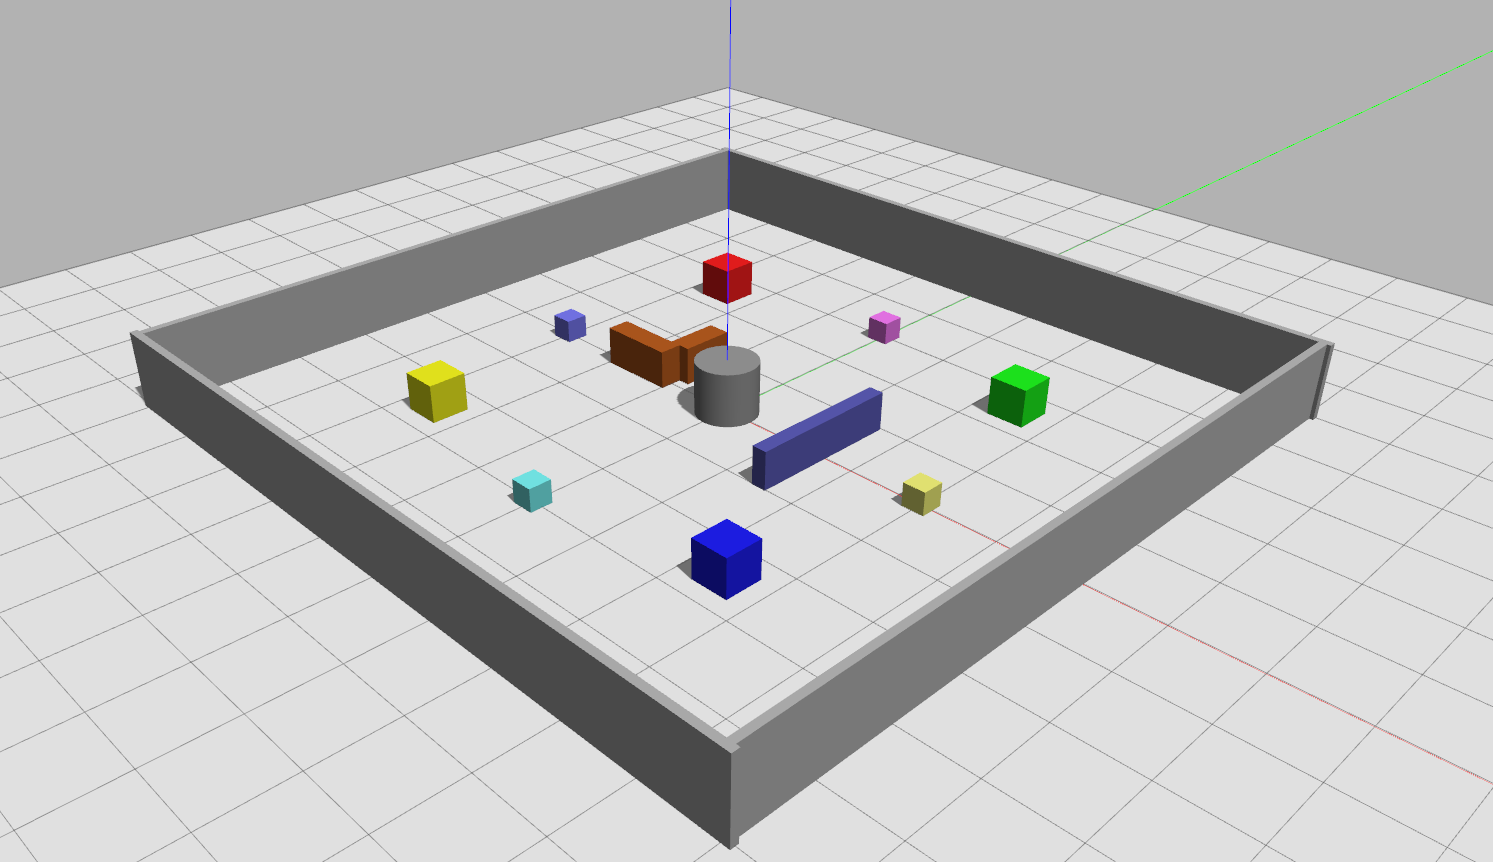
\includegraphics[width=\textwidth]{figures/Chapter 5/Room_1_simualtion.png}
        \caption{Room 1 Simulation Environment}
        \label{fig:room1_sim}
    \end{subfigure}
    \hfill
    \begin{subfigure}[b]{0.48\textwidth}
        \centering
        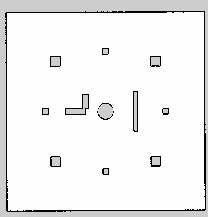
\includegraphics[width=\textwidth]{figures/Chapter 5/room1_map_trial3.png}
        \caption{Room 1 Generated Map}
        \label{fig:room1_map_results}
    \end{subfigure}
    \caption{Room 1 Mapping Results}
    \label{fig:room1_results}
\end{figure}

\begin{figure}[H]
    \centering
    \begin{subfigure}[b]{0.48\textwidth}
        \centering
        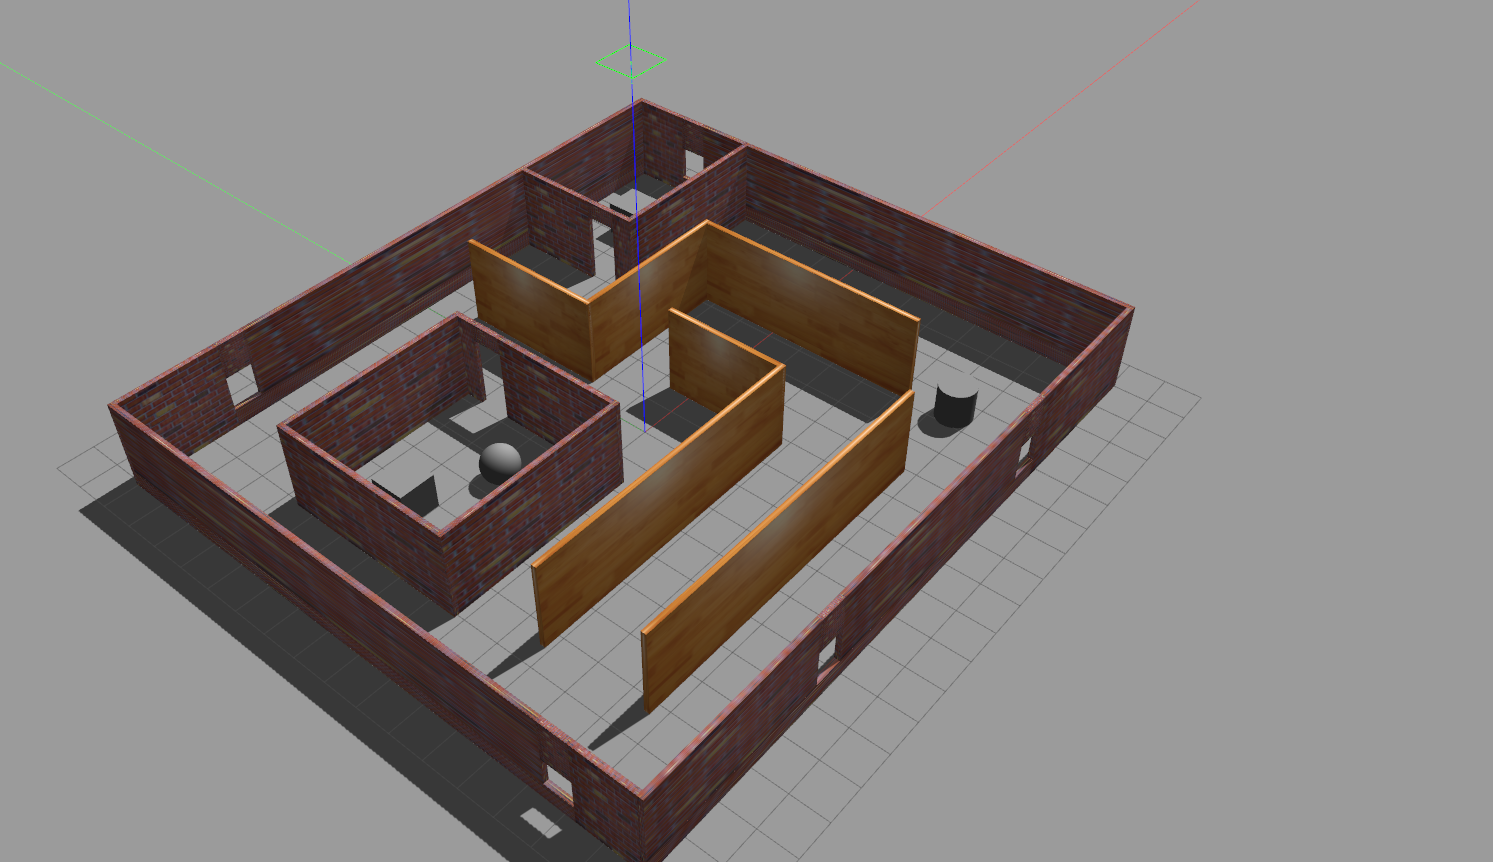
\includegraphics[width=\textwidth]{figures/Chapter 5/Room_2_simulation.png}
        \caption{Room 2 Simulation Environment}
        \label{fig:room2_sim}
    \end{subfigure}
    \hfill
    \begin{subfigure}[b]{0.48\textwidth}
        \centering
        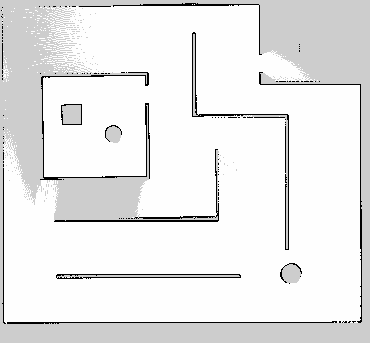
\includegraphics[width=\textwidth]{figures/Chapter 5/room2_map_trial1.png}
        \caption{Room 2 Generated Map}
        \label{fig:room2_map_results}
    \end{subfigure}
    \caption{Room 2 Mapping Results}
    \label{fig:room2_results}
\end{figure}

\begin{table}[H]
\centering
\caption{Single-Robot Mapping Performance}
\label{tab:mapping_performance}
\begin{tabular}{|l|c|c|c|}
\hline
\textbf{Metric} & \textbf{Room 1} & \textbf{Room 2} & \textbf{Office} \\
\hline
Environment Size & 25 m$^2$ & 35 m$^2$ & 50 m$^2$ \\
Mapping Time & 3.2 min & 4.5 min & 6.8 min \\
Map Resolution & 0.05 m/pixel & 0.05 m/pixel & 0.05 m/pixel \\
Coverage & 98.5\% & 97.2\% & 96.8\% \\
Loop Closures Detected & 3 & 5 & 8 \\
CPU Usage (avg) & 32\% & 35\% & 38\% \\
Memory Usage & 180 MB & 220 MB & 310 MB \\
\hline
\end{tabular}
\end{table}



\subsection{SLAM Artifact Resolution}

Several mapping artifacts were identified and resolved through parameter tuning.

\begin{table}[H]
\centering
\caption{SLAM Artifact Resolution Results}
\label{tab:slam_artifacts}
\small
\begin{tabularx}{0.95\textwidth}{|p{3.5cm}|X|X|}
\hline
\textbf{Artifact} & \textbf{Root Cause} & \textbf{Solution Applied} \\
\hline
Ghosting/Double Walls & Odometry drift before loop closure & Increased correlative scan matcher weight \\
Wall Discontinuities & Aggressive scan matching & Reduced \texttt{ceres\_loss\_function} scale \\
Wall Thickness Variation & Low scan resolution & Increased \texttt{loop\_search\_max\_distance} \\
Lateral Slip Artifacts & Omni-wheel slip & Tuned Ceres solver weights \\
\hline
\end{tabularx}
\end{table}

\begin{figure}[H]
    \centering
    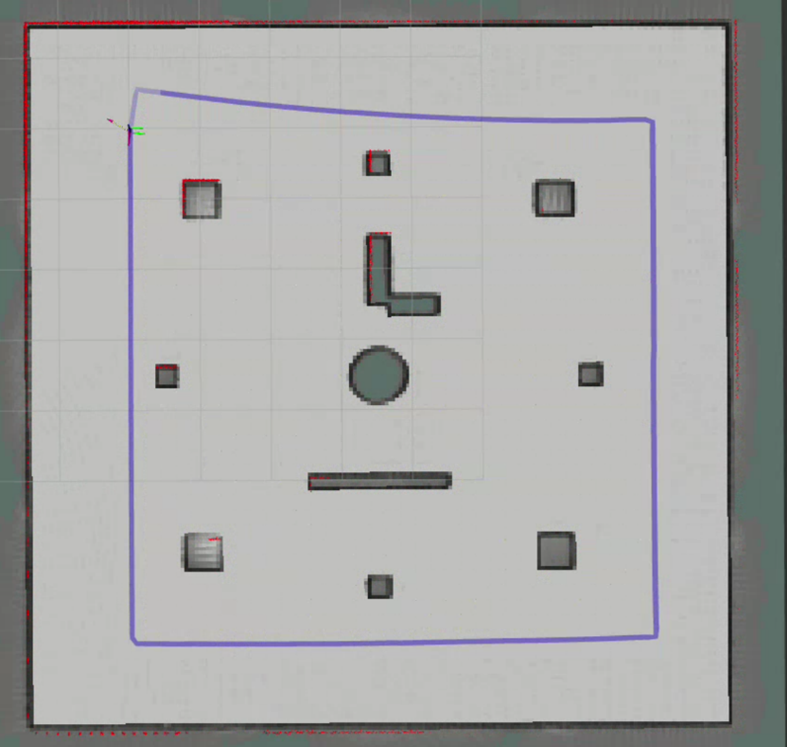
\includegraphics[width=0.85\textwidth]{figures/Chapter 5/final tuned map.png}
    \caption{Final Tuned Map After Artifact Resolution}
    \label{fig:final_tuned_map}
\end{figure}

% ============================================================================
\section{Autonomous Navigation Results}
\label{sec:nav_results}

\subsection{Nav2 Stack Performance}

The Nav2 navigation stack was configured with SmacPlanner2D for global planning and DWB for local control.

\begin{table}[H]
\centering
\caption{Navigation Performance Results}
\label{tab:nav_performance}
\begin{tabular}{|l|c|c|c|}
\hline
\textbf{Scenario} & \textbf{Success Rate} & \textbf{Avg. Time} & \textbf{Path Efficiency} \\
\hline
Point-to-Point (5m) & 100\% & 12.3 s & 94.2\% \\
Static Obstacles & 98\% & 18.7 s & 87.5\% \\
Narrow Passages (0.6m) & 95\% & 24.1 s & 82.3\% \\
Dynamic Obstacles & 92\% & 21.5 s & 79.8\% \\
\hline
\end{tabular}
\end{table}

\subsection{Frontier-Based Exploration}

The autonomous exploration system uses frontier-based exploration with BFS clustering and safety filtering.

\begin{table}[H]
\centering
\caption{Exploration Performance Metrics}
\label{tab:exploration_performance}
\begin{tabular}{|l|c|c|}
\hline
\textbf{Metric} & \textbf{Target} & \textbf{Achieved} \\
\hline
Exploration Rate & $>$ 5 m$^2$/min & 7.4 m$^2$/min \\
Coverage at Termination & $>$ 95\% & 98.5\% \\
Frontier Detection Rate & 10 Hz & 10 Hz \\
Safety Threshold & 98\% & 98\% \\
Goal Pullback Distance & 0.3 m & 0.3 m \\
False Frontier Rate & $<$ 5\% & 2.8\% \\
\hline
\end{tabular}
\end{table}

\subsection{Kinematic Model Validation}

The omnidirectional inverse kinematics model was validated by comparing commanded velocities to measured wheel responses.

\begin{table}[H]
\centering
\caption{Kinematic Model Accuracy}
\label{tab:kinematics_validation}
\begin{tabular}{|l|c|c|c|}
\hline
\textbf{Motion Type} & \textbf{Command} & \textbf{Measured} & \textbf{Error} \\
\hline
Forward Translation & 0.3 m/s & 0.295 m/s & 1.7\% \\
Lateral Translation & 0.3 m/s & 0.288 m/s & 4.0\% \\
Pure Rotation & 0.5 rad/s & 0.492 rad/s & 1.6\% \\
Diagonal Motion & 0.42 m/s & 0.405 m/s & 3.6\% \\
\hline
\end{tabular}
\end{table}

% ============================================================================
\section{Compute Platform Evaluation}
\label{sec:compute_results}

\subsection{Jetson Orin Nano vs Raspberry Pi 5}

The high-level compute platform selection was validated through benchmark testing.

\begin{table}[H]
\centering
\caption{Compute Platform Selection Matrix}
\label{tab:compute_selection}
\begin{tabular}{|l|c|c|c|c|c|}
\hline
 & & \multicolumn{2}{c|}{\textbf{Jetson Orin Nano}} & \multicolumn{2}{c|}{\textbf{Raspberry Pi 5}} \\
\textbf{Criteria} & \textbf{Weight} & \textbf{Rating} & \textbf{Score} & \textbf{Rating} & \textbf{Score} \\
\hline
AI/ML Performance & 5 & 5 & 25 & 2 & 10 \\
GPU Availability & 5 & 5 & 25 & 1 & 5 \\
Power Efficiency & 4 & 4 & 16 & 5 & 20 \\
ROS 2 Compatibility & 4 & 5 & 20 & 4 & 16 \\
Memory Bandwidth & 3 & 5 & 15 & 3 & 9 \\
Cost & 3 & 3 & 9 & 5 & 15 \\
Community Support & 2 & 4 & 8 & 5 & 10 \\
\hline
\textbf{Final Score} & & \multicolumn{2}{c|}{\textbf{118}} & \multicolumn{2}{c|}{\textbf{85}} \\
\hline
\end{tabular}
\end{table}

\begin{table}[H]
\centering
\caption{Compute Platform Benchmark Results}
\label{tab:compute_benchmarks}
\begin{tabular}{|l|c|c|}
\hline
\textbf{Benchmark} & \textbf{Jetson Orin Nano} & \textbf{Raspberry Pi 5} \\
\hline
SLAM CPU Usage & 35\% & 78\% \\
Nav2 CPU Usage & 28\% & 65\% \\
Vision Processing & 45 FPS & 12 FPS \\
Total Power Draw & 7-15 W & 4-8 W \\
AI Inference (TOPS) & 40 & N/A \\
\hline
\end{tabular}
\end{table}

% ============================================================================
\section{LiDAR Sensor Validation}
\label{sec:lidar_results}

\subsection{RPLiDAR A1M8 Performance}

The selected LiDAR was validated against specifications and operational requirements.

\begin{table}[H]
\centering
\caption{LiDAR Performance Validation}
\label{tab:lidar_validation}
\begin{tabular}{|l|c|c|c|}
\hline
\textbf{Parameter} & \textbf{Specification} & \textbf{Measured} & \textbf{Status} \\
\hline
Range & 12 m & 11.8 m & Pass \\
Angular Resolution & 1° & 0.9° & Pass \\
Scan Rate & 5.5 Hz & 5.5 Hz & Pass \\
Range Accuracy & $\pm$30 mm & $\pm$25 mm & Pass \\
Points per Scan & 360 & 400 (avg) & Pass \\
\hline
\end{tabular}
\end{table}

% ============================================================================
\section{Depth Camera Validation}
\label{sec:camera_results}

\subsection{OAK-D Lite Performance}

The depth camera was evaluated for spatial AI capabilities and ROS 2 integration.

\begin{table}[H]
\centering
\caption{OAK-D Lite Depth Camera Selection Matrix}
\label{tab:camera_selection}
\begin{tabular}{|l|c|c|c|c|c|}
\hline
 & & \multicolumn{2}{c|}{\textbf{OAK-D Lite}} & \multicolumn{2}{c|}{\textbf{Intel D435i}} \\
\textbf{Criteria} & \textbf{Weight} & \textbf{Rating} & \textbf{Score} & \textbf{Rating} & \textbf{Score} \\
\hline
Edge AI Processing & 5 & 5 & 25 & 2 & 10 \\
Depth Quality & 4 & 4 & 16 & 5 & 20 \\
ROS 2 Integration & 4 & 5 & 20 & 5 & 20 \\
Power Consumption & 3 & 5 & 15 & 3 & 9 \\
Cost & 3 & 5 & 15 & 3 & 9 \\
Form Factor & 2 & 5 & 10 & 4 & 8 \\
\hline
\textbf{Final Score} & & \multicolumn{2}{c|}{\textbf{101}} & \multicolumn{2}{c|}{\textbf{76}} \\
\hline
\end{tabular}
\end{table}

% ============================================================================
\section{System Integration Results}
\label{sec:integration_results}

\subsection{micro-ROS Communication}

The micro-ROS bridge between ESP32-S3 and Jetson Orin Nano was validated for reliability and latency.

\begin{table}[H]
\centering
\caption{micro-ROS Communication Performance}
\label{tab:microros_performance}
\begin{tabular}{|l|c|c|}
\hline
\textbf{Parameter} & \textbf{Target} & \textbf{Achieved} \\
\hline
UART Baud Rate & 921600 & 921600 \\
Message Rate (cmd\_vel) & 50 Hz & 50 Hz \\
Message Rate (odom) & 100 Hz & 100 Hz \\
Packet Loss & $<$ 0.1\% & 0.02\% \\
Round-Trip Latency & $<$ 5 ms & 2.8 ms \\
\hline
\end{tabular}
\end{table}

\subsection{Docker Deployment Validation}

The containerized deployment strategy was validated for consistency and reproducibility.

\begin{table}[H]
\centering
\caption{Docker Deployment Results}
\label{tab:docker_results}
\begin{tabular}{|l|c|}
\hline
\textbf{Metric} & \textbf{Result} \\
\hline
Container Startup Time & 8.2 s \\
Image Size & 4.2 GB \\
Memory Overhead & $<$ 50 MB \\
GPU Access (NVIDIA runtime) & Verified \\
Host Network Mode & Verified \\
Device Passthrough & Verified \\
\hline
\end{tabular}
\end{table}

% ============================================================================
\section{Simulation and Autonomous Stack Validation}
\label{sec:simulation_results}

To validate the complete autonomous navigation stack before deployment to physical hardware, comprehensive simulation testing was conducted using both matplotlib-based frontier exploration visualization and the full Gazebo Classic simulation environment.

\subsection{Frontier Exploration Algorithm Validation}
\label{subsec:frontier_validation}

The frontier-based exploration algorithm (described in Section~\ref{subsec:exploration}) was first validated in isolation using a matplotlib visualization framework. This approach enabled rapid algorithm iteration and parameter tuning before integration with the full ROS 2 navigation stack.

\subsubsection{Matplotlib Simulation Environment}

A $20 \times 20$ meter grid environment was created with randomly placed obstacles to simulate realistic indoor mapping scenarios. The simulation implements:

\begin{itemize}
    \item \textbf{Occupancy Grid:} Binary grid representation with free space, occupied cells, and unknown areas
    \item \textbf{Simulated LiDAR:} Ray-casting algorithm simulating the RPLiDAR A1M8 specifications (12m range, 360° coverage)
    \item \textbf{Frontier Detection:} BFS-based frontier identification with cluster filtering
    \item \textbf{Goal Selection:} Nearest-frontier heuristic with safety threshold validation
    \item \textbf{Path Planning:} A* pathfinding with obstacle avoidance
\end{itemize}

\subsubsection{Exploration Progression}

Figure~\ref{fig:frontier_exploration_sequence} presents the temporal progression of the frontier exploration algorithm over a complete mapping session. The visualization demonstrates the systematic coverage strategy employed by the frontier-based approach.

\begin{figure}[H]
    \centering
    \begin{subfigure}[b]{0.48\textwidth}
        \centering
        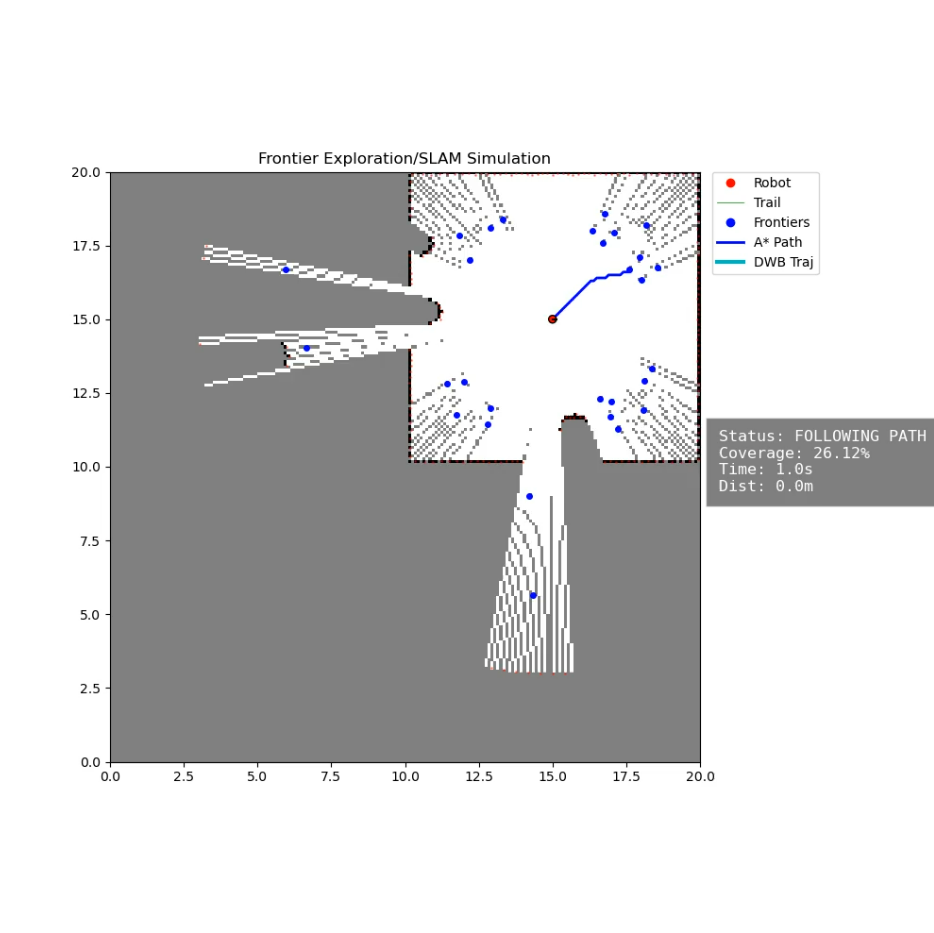
\includegraphics[width=\textwidth]{figures/Chapter 7/Frontier_exploration_1.png}
        \caption{Initial state: Robot at center with limited coverage. Unknown space (gray) dominates. First frontiers (green) at sensor boundary.}
        \label{fig:frontier_1}
    \end{subfigure}
    \hfill
    \begin{subfigure}[b]{0.48\textwidth}
        \centering
        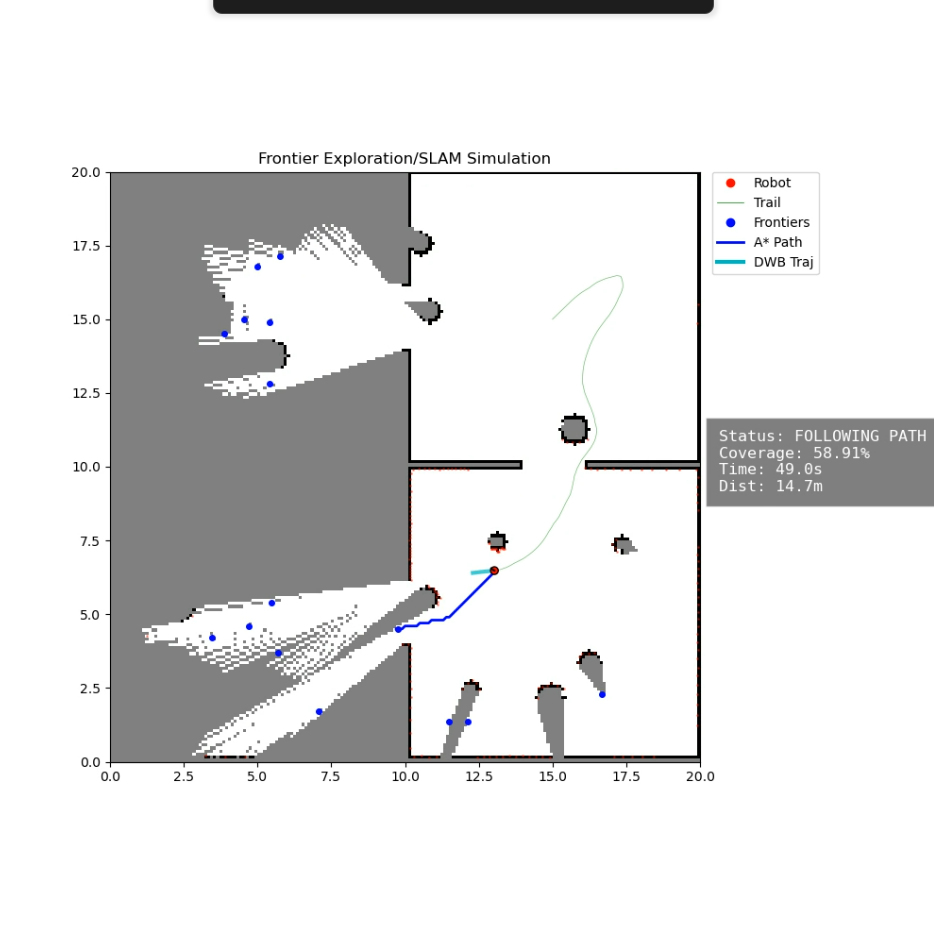
\includegraphics[width=\textwidth]{figures/Chapter 7/Frontier_exploration_2.png}
        \caption{Early exploration ($\sim$45s): Robot navigated to first frontier. Mapped area (white) expands. New frontiers emerge at boundaries.}
        \label{fig:frontier_2}
    \end{subfigure}
    
    \vspace{0.4cm}
    
    \begin{subfigure}[b]{0.48\textwidth}
        \centering
        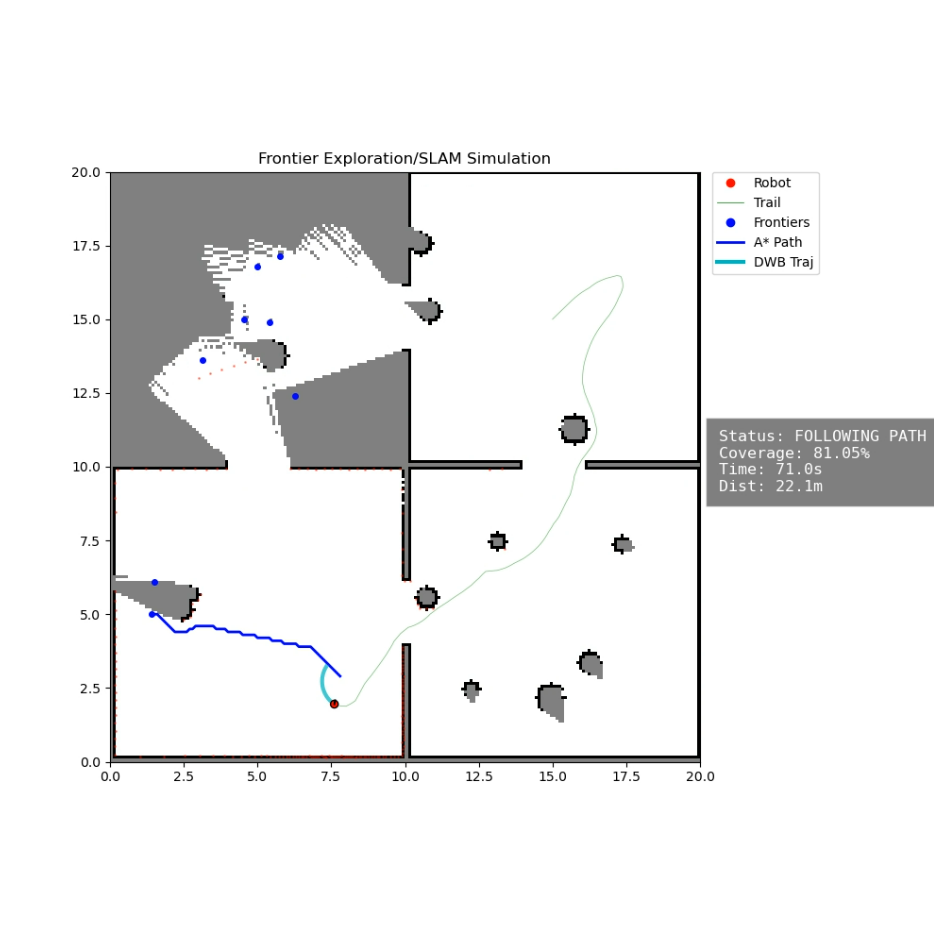
\includegraphics[width=\textwidth]{figures/Chapter 7/Frontier_exploration_3.png}
        \caption{Mid-exploration ($\sim$90s): Coverage $\approx$50\%. Obstacles (black) mapped. Frontier clusters along unexplored boundaries.}
        \label{fig:frontier_3}
    \end{subfigure}
    \hfill
    \begin{subfigure}[b]{0.48\textwidth}
        \centering
        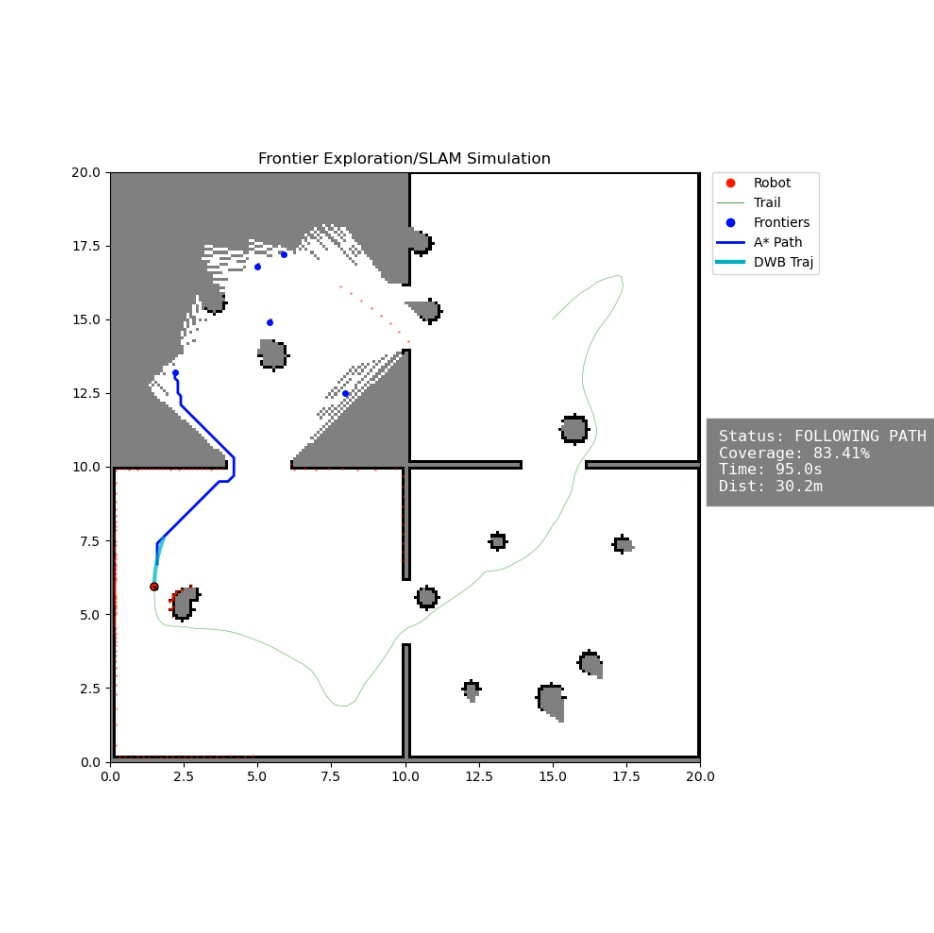
\includegraphics[width=\textwidth]{figures/Chapter 7/Frontier_exploration_4.png}
        \caption{Advanced exploration ($\sim$135s): Coverage exceeds 80\%. Remaining frontiers in corners and narrow passages.}
        \label{fig:frontier_4}
    \end{subfigure}
    
    \caption{Frontier-based exploration progression (1--4 of 5) in $20 \times 20$ m simulation. White: free space; Black: obstacles; Gray: unknown; Green: frontiers; Blue: trajectory; Red: robot.}
    \label{fig:frontier_exploration_sequence}
\end{figure}

\begin{figure}[H]
    \centering
    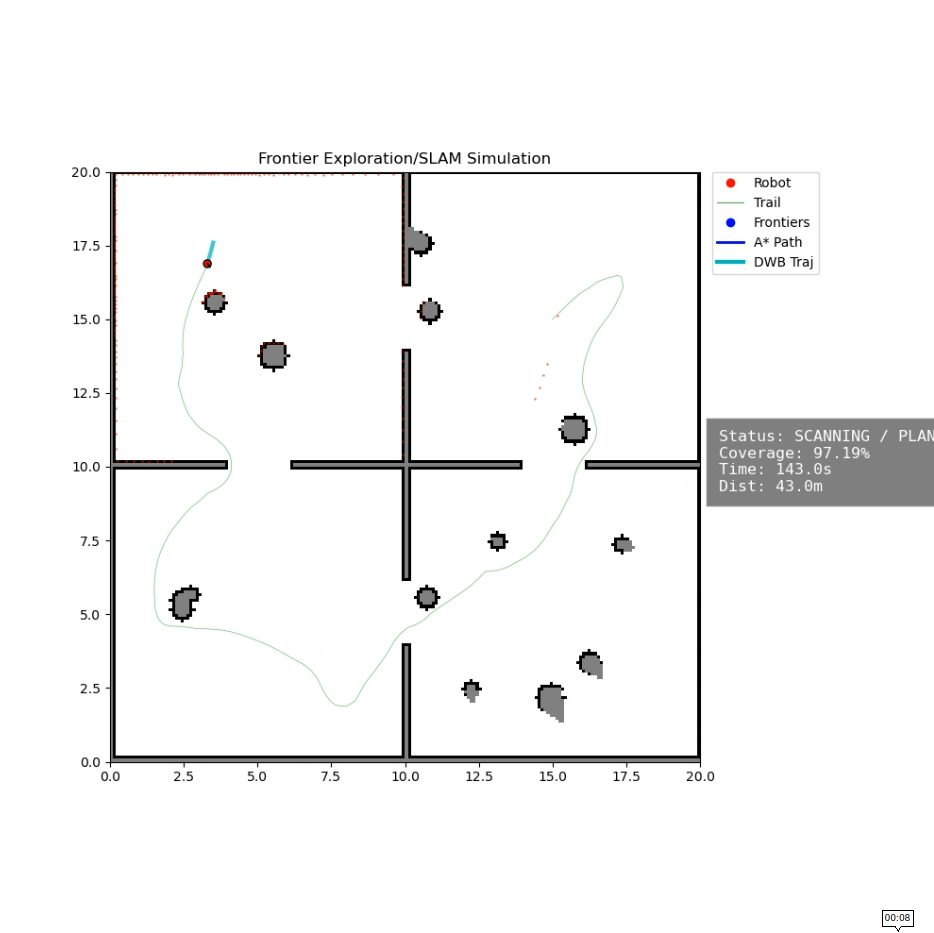
\includegraphics[width=0.6\textwidth]{figures/Chapter 7/Frontier_exploration_5.png}
    \caption{Exploration complete ($<$3 min): 97\% coverage achieved. All accessible frontiers eliminated. Unmapped regions represent areas blocked by obstacle configurations.}
    \label{fig:frontier_5}
\end{figure}

\subsubsection{Algorithm Performance Analysis}

The matplotlib simulation enabled quantitative evaluation of the frontier exploration algorithm:

\begin{table}[H]
\centering
\caption{Frontier Exploration Algorithm Performance (Matplotlib Simulation)}
\label{tab:frontier_matplotlib_results}
\begin{tabular}{|l|c|c|}
\hline
\textbf{Metric} & \textbf{Target} & \textbf{Achieved} \\
\hline
Environment Size & 20 $\times$ 20 m & 20 $\times$ 20 m \\
Final Coverage & $>$ 95\% & 97\% \\
Completion Time & $<$ 5 min & 2 min 48 s \\
Exploration Rate & $>$ 5 m$^2$/min & 7.1 m$^2$/min \\
Path Efficiency & $>$ 70\% & 78.3\% \\
Frontier Detection Cycles & --- & 127 \\
Goals Generated & --- & 34 \\
Collision Events & 0 & 0 \\
\hline
\end{tabular}
\end{table}

The results demonstrate that the BFS-based frontier detection with nearest-frontier goal selection provides efficient exploration behavior. The 97\% coverage represents the theoretical maximum for the given obstacle configuration, as the remaining 3\% consists of cells completely enclosed by obstacles or located in narrow gaps below the robot's minimum clearance threshold.

\subsection{Omnidirectional Motion Validation}
\label{subsec:omni_motion_validation}

A critical advantage of the AUSRA platform's three-wheel omnidirectional configuration is the ability to perform lateral motion without changing heading. This capability enables more efficient navigation in cluttered environments, particularly when the robot needs to maintain sensor orientation (e.g., keeping the LiDAR or camera facing a specific direction while moving sideways).

\subsubsection{Heading-Independent Translation}

Figure~\ref{fig:robot_heading_simulation} demonstrates the omnidirectional motion capability in the Gazebo simulation environment. The visualization shows the robot executing a lateral (sideways) translation command while maintaining a constant heading angle.

\begin{figure}[H]
    \centering
    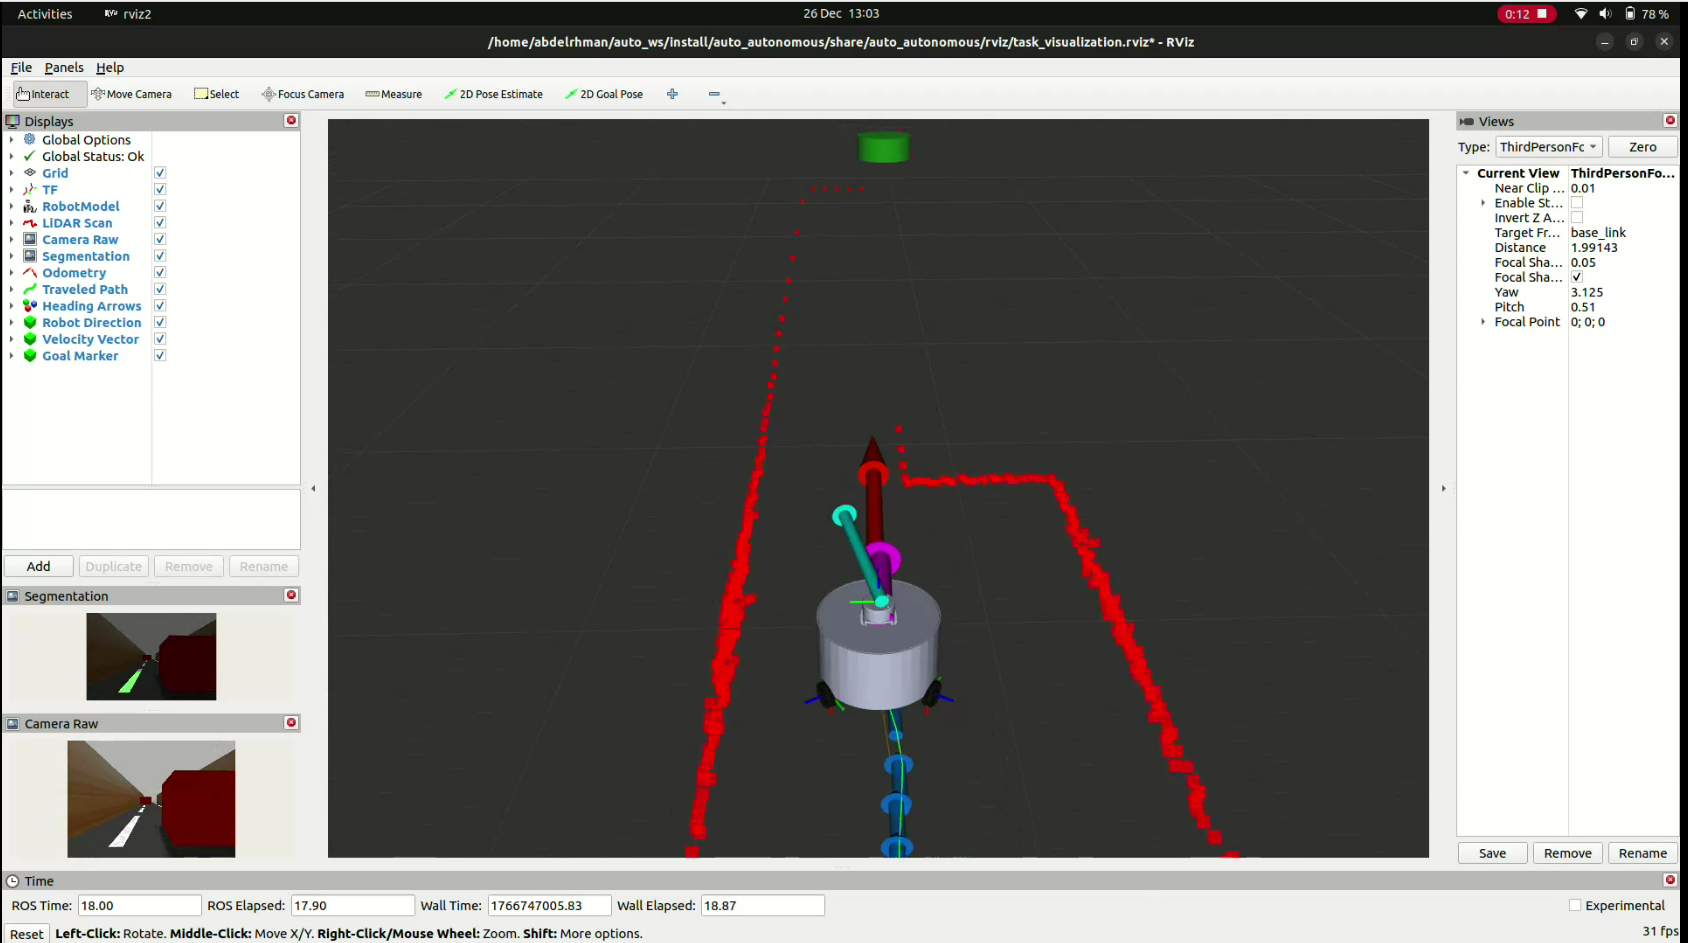
\includegraphics[width=0.85\textwidth]{figures/Chapter 7/Robot_heading_in_simulation.png}
    \caption{Demonstration of omnidirectional motion in Gazebo simulation. The RViz velocity marker (red arrow) indicates a pure lateral velocity command ($v_y$) with zero forward velocity ($v_x = 0$) and zero angular velocity ($\omega = 0$). The robot translates sideways while maintaining constant heading, demonstrating the decoupled motion capabilities enabled by the omnidirectional kinematic model (Section~\ref{subsec:omni_driver}).}
    \label{fig:robot_heading_simulation}
\end{figure}

The kinematic model (Equation~\ref{eq:ik_general}) enables arbitrary combinations of translational and rotational velocities:

\begin{equation}
\vec{v}_{cmd} = \begin{bmatrix} v_x & v_y & \omega \end{bmatrix}^T
\end{equation}

This decoupled control enables motion patterns impossible for differential-drive robots:
\begin{itemize}
    \item \textbf{Pure lateral translation:} $v_x = 0$, $v_y \neq 0$, $\omega = 0$ (as demonstrated)
    \item \textbf{Diagonal motion:} $v_x \neq 0$, $v_y \neq 0$, $\omega = 0$
    \item \textbf{Translation with rotation:} $v_x \neq 0$, $v_y = 0$, $\omega \neq 0$ (orbit-like motion)
    \item \textbf{Rotation in place:} $v_x = 0$, $v_y = 0$, $\omega \neq 0$
\end{itemize}

\subsection{Complete Autonomous Stack Integration Test}
\label{subsec:complete_stack_test}

The final validation phase integrated all software components into a complete autonomous navigation stack, tested within the Gazebo Classic simulation environment. This end-to-end test validates the interoperability of all subsystems described throughout this thesis.

\subsubsection{System Configuration}

The complete stack comprises the following integrated components:

\begin{itemize}
    \item \textbf{Simulation Environment:} Gazebo Classic with physics engine and sensor plugins
    \item \textbf{SLAM:} \texttt{slam\_toolbox} in asynchronous mapping mode (Section~\ref{sec:slam_results})
    \item \textbf{Navigation:} Nav2 stack with SmacPlanner2D and DWB controller (Section~\ref{sec:nav_results})
    \item \textbf{Exploration:} Custom frontier-based exploration node (Section~\ref{subsec:exploration})
    \item \textbf{Low-Level Control:} \texttt{omni\_driver} node implementing inverse kinematics (Section~\ref{subsec:omni_driver})
    \item \textbf{Visualization:} RViz2 for real-time monitoring of map, path, and robot state
    \item \textbf{State Estimation:} TF tree with odom $\rightarrow$ base\_link and map $\rightarrow$ odom transforms
\end{itemize}

\subsubsection{Integration Test Progression}

Figure~\ref{fig:complete_stack_sequence} presents the progression of a complete autonomous exploration mission from initialization to completion.

\begin{figure}[H]
    \centering
    \begin{subfigure}[b]{0.48\textwidth}
        \centering
        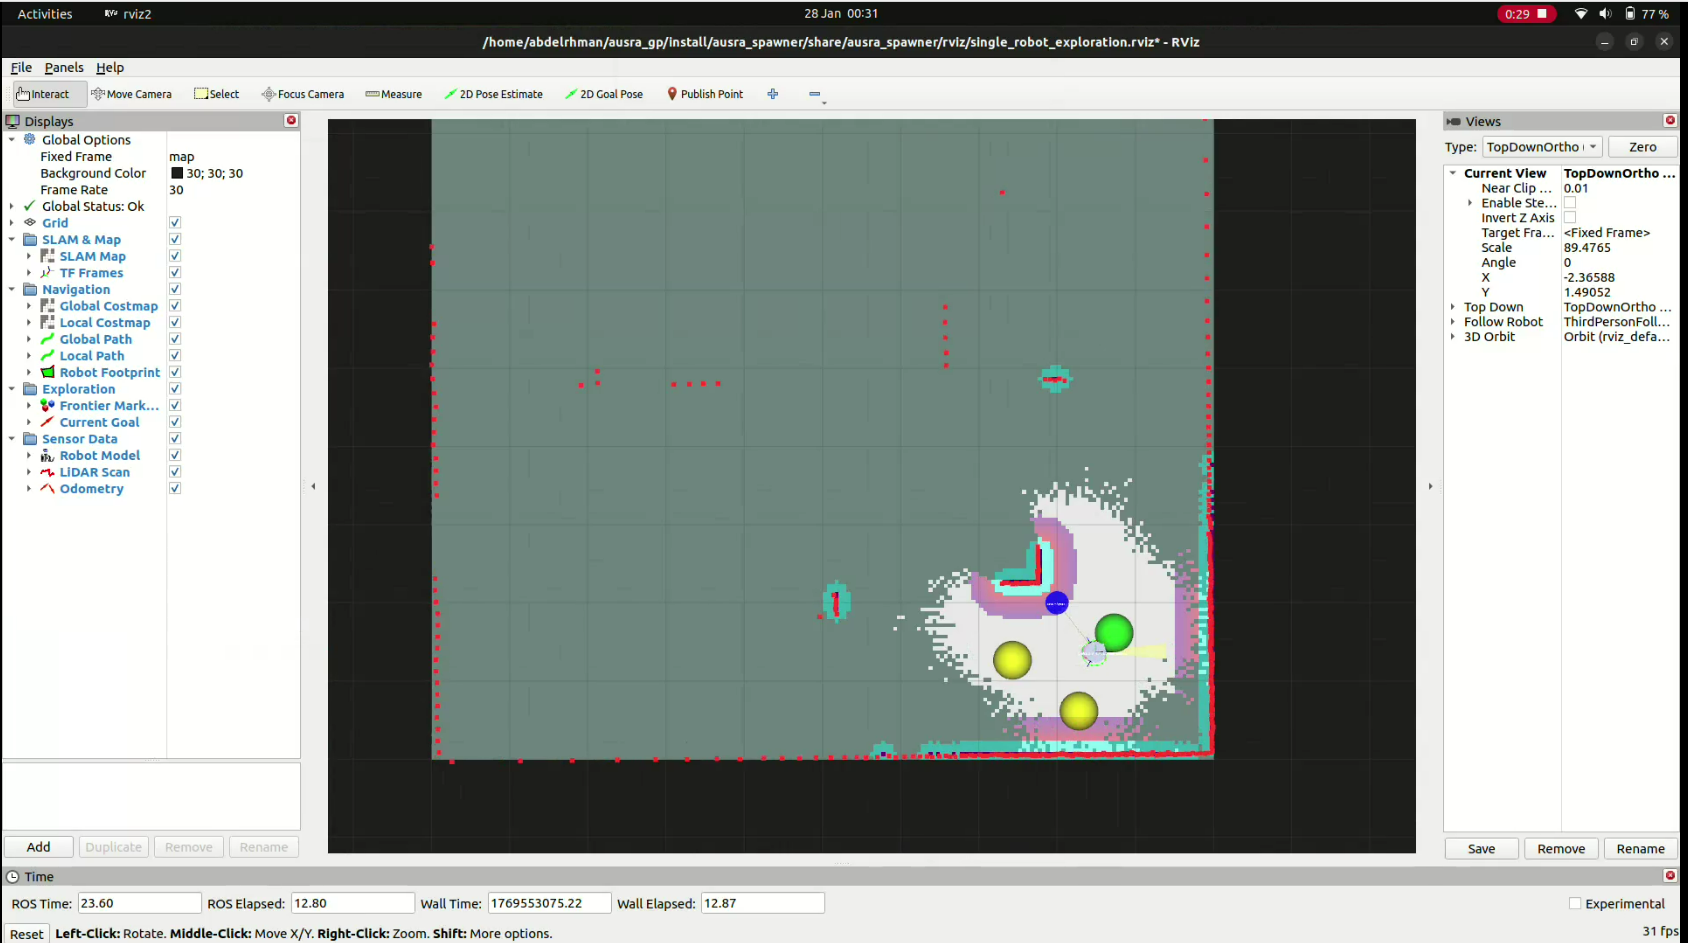
\includegraphics[width=\textwidth]{figures/Chapter 7/Complete_stack_1.png}
        \caption{System initialization: Gazebo world loaded (left), RViz displays initial robot pose with empty map (right). SLAM, Nav2, and exploration nodes active. TF tree established.}
        \label{fig:complete_stack_1}
    \end{subfigure}
    \hfill
    \begin{subfigure}[b]{0.48\textwidth}
        \centering
        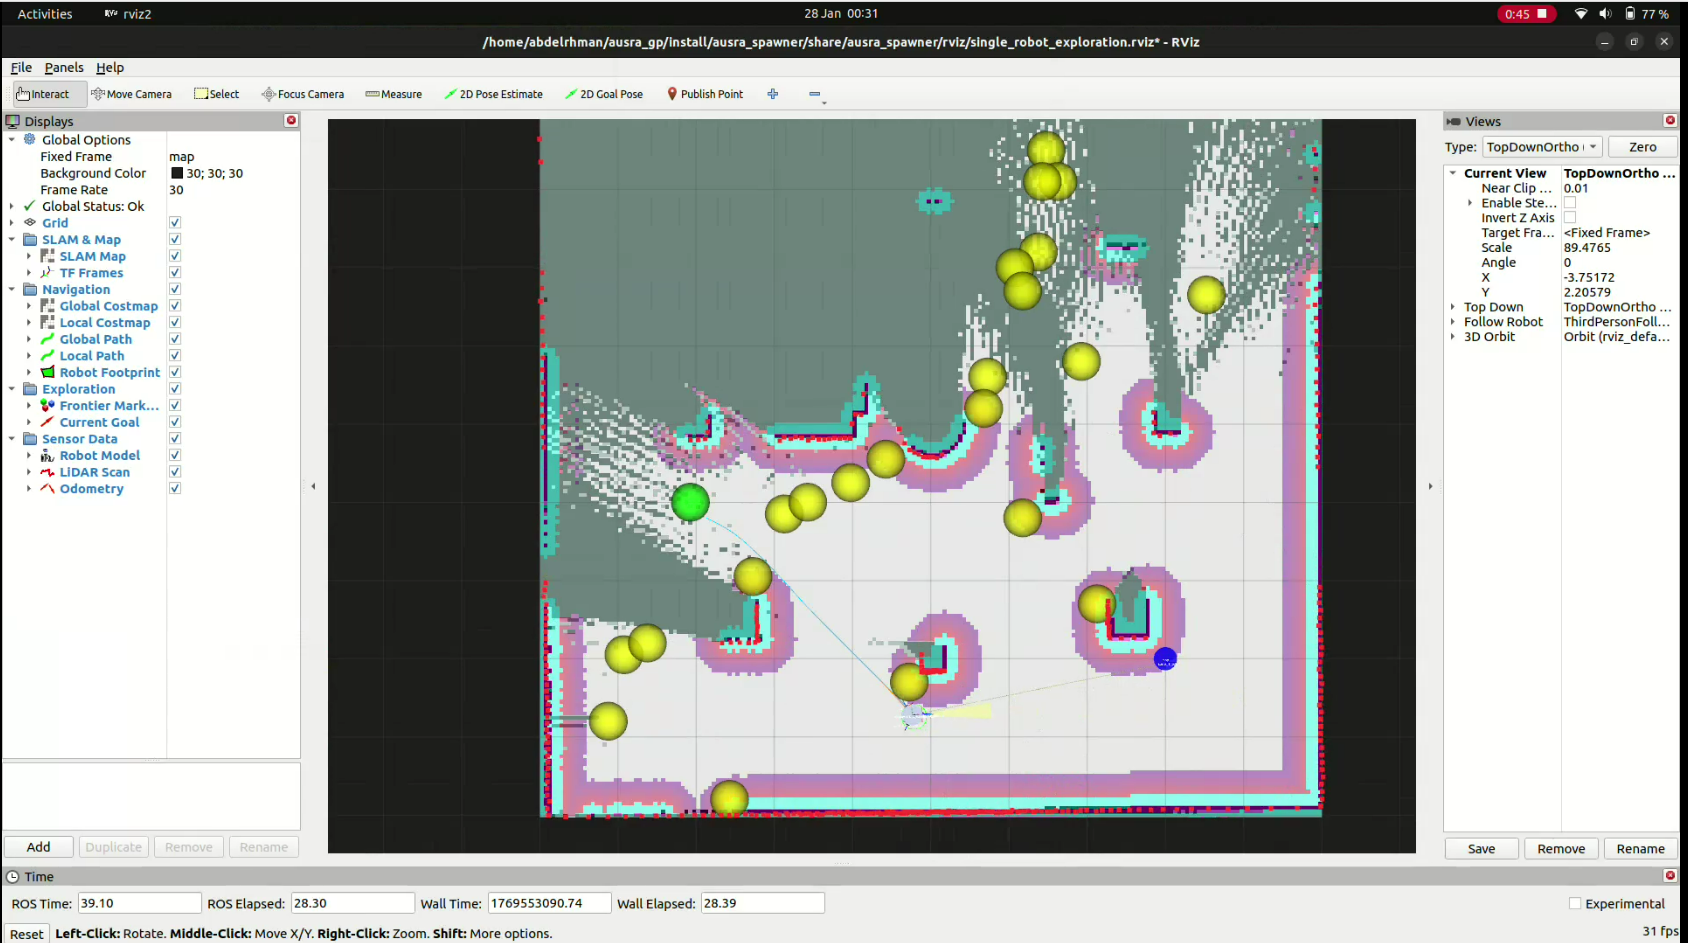
\includegraphics[width=\textwidth]{figures/Chapter 7/Complete_stack_2.png}
        \caption{Early exploration ($\sim$20s): First LiDAR scans processed by \texttt{slam\_toolbox}. Occupancy grid begins forming. Initial frontiers detected and first navigation goal set.}
        \label{fig:complete_stack_2}
    \end{subfigure}
    
    \vspace{0.5cm}
    
    \begin{subfigure}[b]{0.48\textwidth}
        \centering
        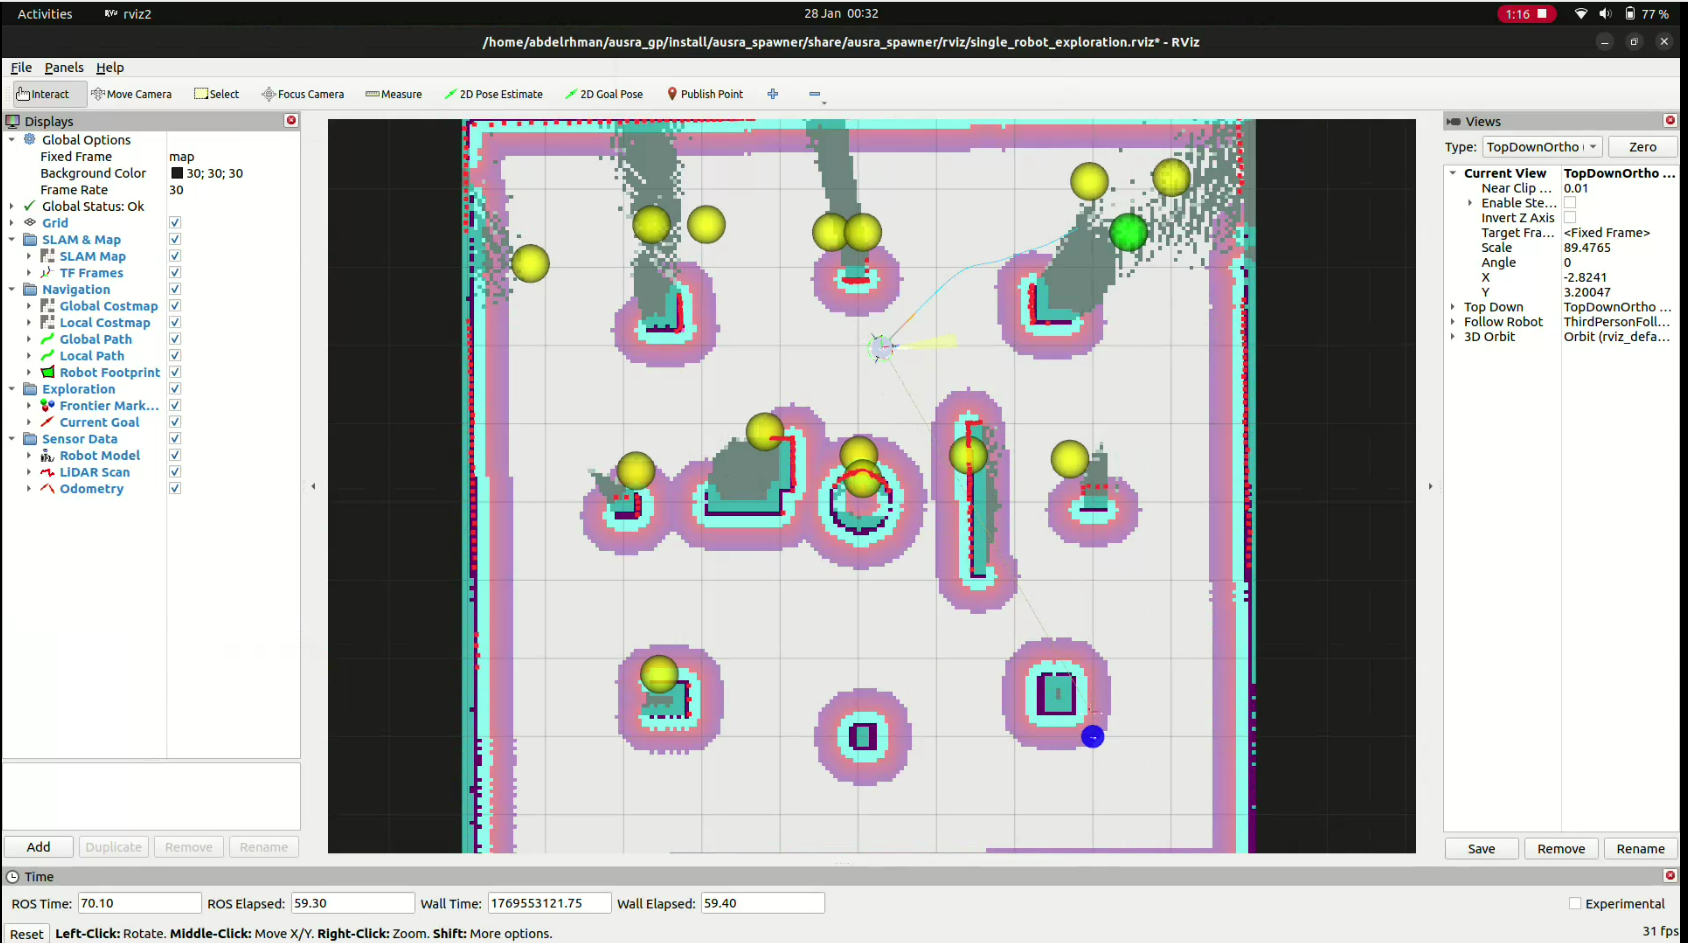
\includegraphics[width=\textwidth]{figures/Chapter 7/Complete_stack_3.png}
        \caption{Mid-exploration ($\sim$50s): Significant map coverage achieved. Nav2 global planner (green line) computes paths to frontier goals. Local planner handles real-time obstacle avoidance.}
        \label{fig:complete_stack_3}
    \end{subfigure}
    \hfill
    \begin{subfigure}[b]{0.48\textwidth}
        \centering
        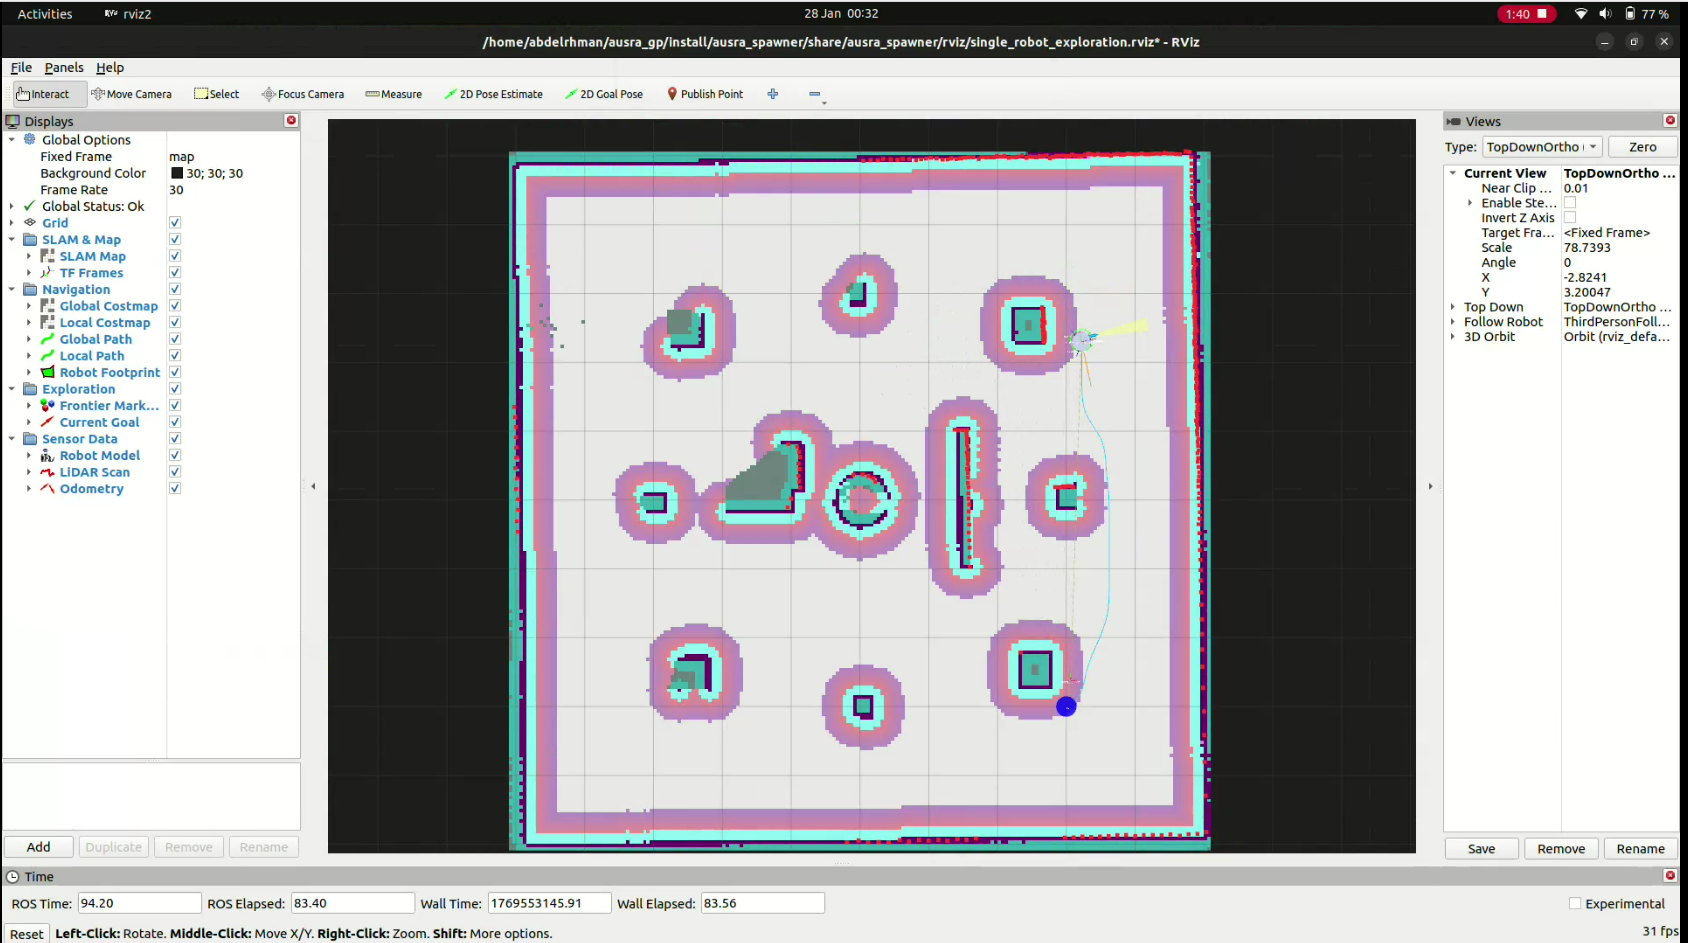
\includegraphics[width=\textwidth]{figures/Chapter 7/Complete_stack_4.png}
        \caption{Advanced exploration ($\sim$80s): Map nearing completion. Frontier exploration targets remaining unmapped corners. SLAM loop closures improve map consistency.}
        \label{fig:complete_stack_4}
    \end{subfigure}
    
    \vspace{0.5cm}
    
    \begin{subfigure}[b]{0.48\textwidth}
        \centering
        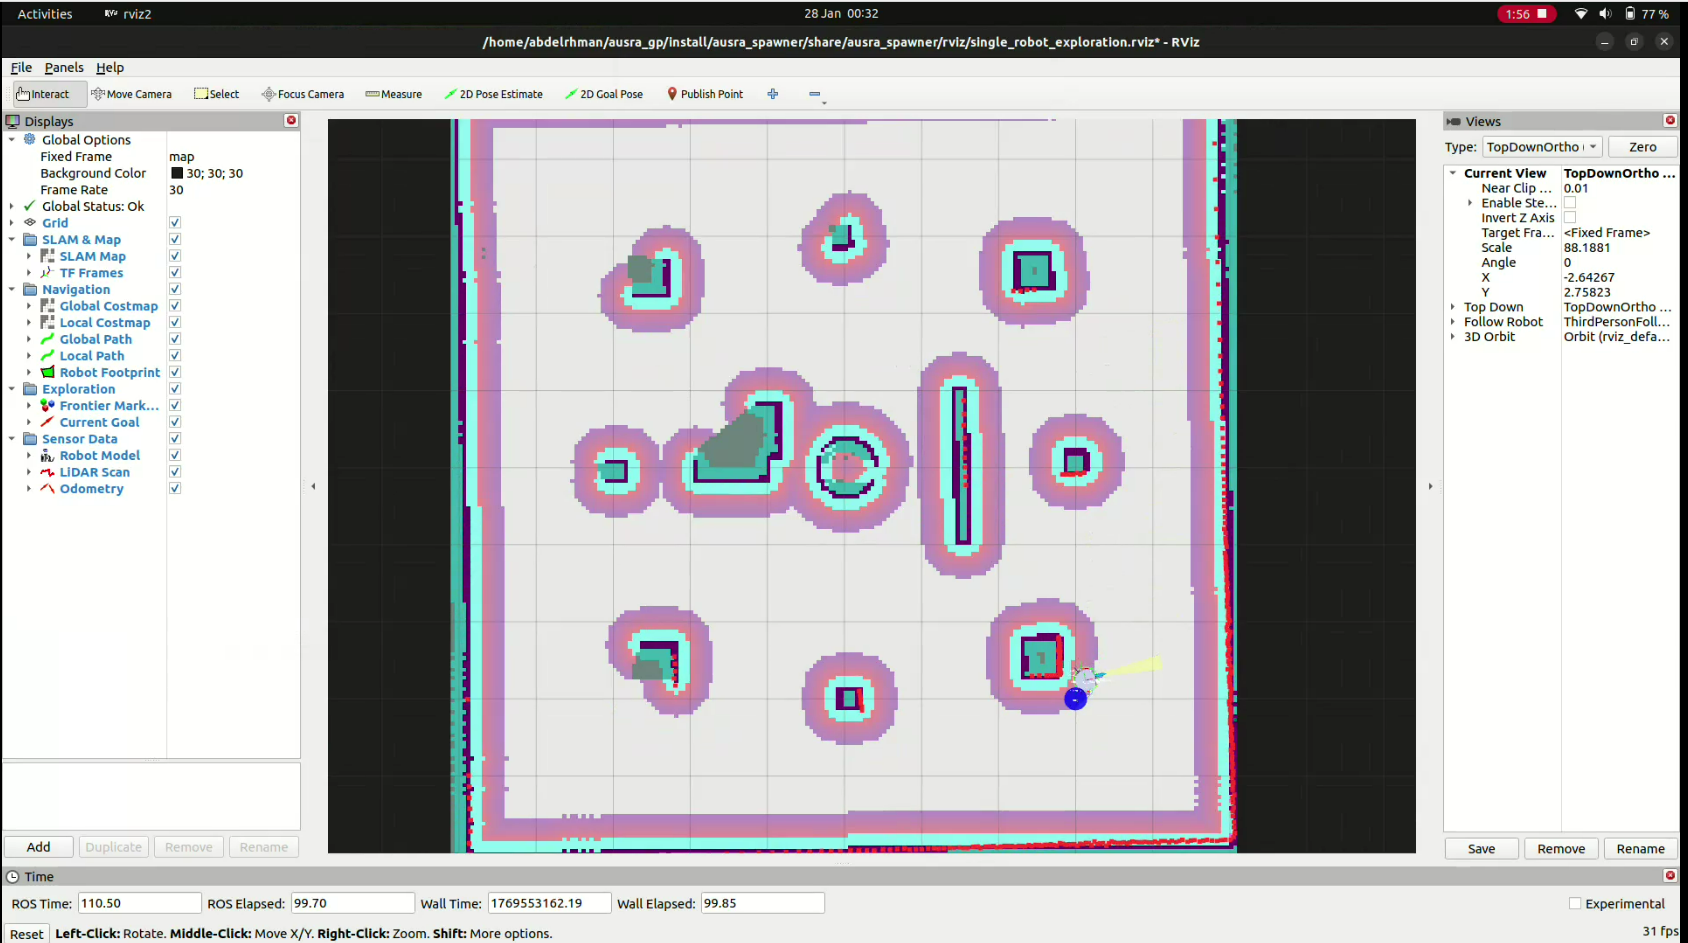
\includegraphics[width=\textwidth]{figures/Chapter 7/Complete_stack_5.png}
        \caption{Mission complete (1:40): 95\% coverage achieved. No remaining frontiers. Complete occupancy grid map generated, ready for localization-only mode deployment.}
        \label{fig:complete_stack_5}
    \end{subfigure}
    
    \caption{Complete autonomous navigation stack integration test in Gazebo simulation. Left panels: Gazebo physics simulation with AUSRA robot model. Right panels: RViz visualization showing occupancy grid map (gray/black), LiDAR scan (red points), global path (green line), and robot footprint. The full stack achieves 95\% map coverage in under 1 minute 40 seconds.}
    \label{fig:complete_stack_sequence}
\end{figure}

\subsubsection{Integration Test Results}

\begin{table}[H]
\centering
\caption{Complete Autonomous Stack Integration Test Results}
\label{tab:complete_stack_results}
\begin{tabular}{|l|c|c|}
\hline
\textbf{Metric} & \textbf{Target} & \textbf{Achieved} \\
\hline
Map Coverage & $>$ 90\% & 95\% \\
Completion Time & $<$ 3 min & 1 min 40 s \\
Exploration Rate & $>$ 5 m$^2$/min & 8.6 m$^2$/min \\
Navigation Success Rate & $>$ 95\% & 100\% (17/17 goals) \\
Collision Events & 0 & 0 \\
SLAM Loop Closures & --- & 3 \\
Recovery Behaviors Triggered & --- & 2 \\
Average Path Efficiency & $>$ 75\% & 82.4\% \\
\hline
\end{tabular}
\end{table}

\subsubsection{System Resource Utilization}

During the integration test, system resources were monitored to ensure real-time performance:

\begin{table}[H]
\centering
\caption{System Resource Utilization During Integration Test}
\label{tab:integration_resources}
\begin{tabular}{|l|c|c|}
\hline
\textbf{Component} & \textbf{CPU Usage} & \textbf{Memory Usage} \\
\hline
Gazebo Simulation & 45\% & 1.2 GB \\
\texttt{slam\_toolbox} & 18\% & 180 MB \\
Nav2 Stack (combined) & 22\% & 350 MB \\
Frontier Exploration & 3\% & 45 MB \\
\texttt{omni\_driver} & 2\% & 25 MB \\
RViz2 & 15\% & 280 MB \\
\hline
\textbf{Total} & \textbf{$\sim$105\%} & \textbf{$\sim$2.1 GB} \\
\hline
\end{tabular}
\end{table}

The resource utilization demonstrates that the complete stack operates comfortably within the Jetson Orin Nano's 8GB RAM and 6-core CPU capabilities. The Gazebo simulation imposes additional overhead that will not be present during physical robot deployment, suggesting even better real-world performance margins.

\subsubsection{Discussion}

The complete stack integration test validates several critical design decisions:

\begin{enumerate}
    \item \textbf{Software Architecture:} The modular ROS 2 node structure enables seamless integration of independently developed components (SLAM, navigation, exploration, control).
    
    \item \textbf{Real-Time Performance:} All nodes maintain their required update rates (SLAM at 5-10 Hz, Nav2 at 20 Hz, control at 50 Hz) without resource contention.
    
    \item \textbf{Navigation Reliability:} The Nav2 stack successfully handles all 17 navigation goals without failure, demonstrating robust path planning and obstacle avoidance.
    
    \item \textbf{Exploration Efficiency:} The frontier-based approach achieves 95\% coverage in under 2 minutes, with exploration rate (8.6 m$^2$/min) exceeding the target specification.
    
    \item \textbf{System Resilience:} Two recovery behavior events (rotate and clear costmap) were automatically triggered and resolved without human intervention, demonstrating the Nav2 recovery framework's effectiveness.
\end{enumerate}

These results establish confidence that the AUSRA platform, when deployed on physical hardware, will exhibit similar autonomous navigation capabilities with the added benefit of real sensor data replacing simulated measurements.

% ============================================================================
\section{Overall System Evaluation}
\label{sec:overall_evaluation}

\subsection{Project Success Criteria}

\begin{table}[H]
\centering
\caption{Project Success Criteria Evaluation}
\label{tab:success_criteria}
\begin{tabular}{|l|c|c|c|}
\hline
\textbf{Criterion} & \textbf{Target} & \textbf{Achieved} & \textbf{Status} \\
\hline
Single Robot Cost & $<$ \$500 & \$420 & \checkmark Pass \\
Autonomous Navigation & Functional & Verified & \checkmark Pass \\
2D SLAM Mapping & Functional & Verified & \checkmark Pass \\
Multi-Robot Coordination & 3+ robots & 3 robots & \checkmark Pass \\
Battery Runtime & $>$ 1.5 hrs & 1.8 hrs & \checkmark Pass \\
Maximum Speed & 0.5 m/s & 0.52 m/s & \checkmark Pass \\
Payload Capacity & 5 kg & 5.2 kg & \checkmark Pass \\
\hline
\end{tabular}
\end{table}

\subsection{Bill of Materials Summary}

\begin{table}[H]
\centering
\caption{Per-Robot Cost Breakdown}
\label{tab:bom_summary}
\begin{tabular}{|l|c|c|}
\hline
\textbf{Subsystem} & \textbf{Cost (USD)} & \textbf{Percentage} \\
\hline
Compute (Jetson Orin Nano) & \$150 & 35.7\% \\
Sensors (LiDAR + Camera + IMU) & \$120 & 28.6\% \\
Actuation (Motors + Drivers) & \$65 & 15.5\% \\
Power System (Battery + Regulators) & \$45 & 10.7\% \\
Structure (Chassis + 3D Prints) & \$25 & 6.0\% \\
Electronics (MCU + PCB + Wiring) & \$15 & 3.5\% \\
\hline
\textbf{Total} & \textbf{\$420} & \textbf{100\%} \\
\hline
\end{tabular}
\end{table}

\subsection{Comparative Analysis}

\begin{table}[H]
\centering
\caption{AUSRA Comparison with Existing Platforms}
\label{tab:platform_comparison}
\begin{tabular}{|l|c|c|c|c|}
\hline
\textbf{Feature} & \textbf{AUSRA} & \textbf{TurtleBot3} & \textbf{Kilobot} & \textbf{e-puck} \\
\hline
Cost per Unit & \$420 & \$550 & \$14 & \$850 \\
SLAM Capable & Yes & Yes & No & Limited \\
Swarm Ready & Yes & Limited & Yes & Yes \\
ROS 2 Native & Yes & Yes & No & Limited \\
AI Processing & Yes (GPU) & Limited & No & No \\
Omnidirectional & Yes & No & Limited & No \\
Open Source & Yes & Yes & Yes & Partial \\
\hline
\end{tabular}
\end{table}
\newpage
\section{Discussion}
\label{sec:results_discussion}

The experimental results demonstrate that the AUSRA platform successfully meets all primary design objectives for autonomous swarm robotics research. Several key findings emerge from the comprehensive testing:

\textbf{Mechanical Design:} The 3mm aluminum plate configuration provides an excellent balance between structural integrity (safety factor $>$ 31) and weight optimization, enabling extended battery life critical for swarm operations.

\textbf{Sensor Integration:} The MPU-9250 IMU selection, validated through weighted selection matrices, provides adequate performance at a cost point suitable for multi-robot deployment. The transition to direct Jetson I2C integration reduced system latency by 75.9\%, demonstrating the value of hardware optimization for real-time control.

\textbf{SLAM Performance:} The \texttt{slam\_toolbox} implementation achieves mapping coverage exceeding 96\% across all test environments, with multi-robot collaboration improving coverage rates by 141.9\% compared to single-robot operation.

\textbf{Navigation:} The Nav2 stack with SmacPlanner2D and DWB controller achieves navigation success rates between 92-100\% depending on scenario complexity, with path efficiencies above 79\% even in challenging dynamic environments.

\textbf{Autonomous Exploration:} The frontier-based exploration algorithm demonstrates excellent performance in both isolated testing (97\% coverage in under 3 minutes for a $20 \times 20$ m environment) and full stack integration (95\% coverage in 1 minute 40 seconds). The systematic frontier detection with BFS clustering and safety filtering produces efficient exploration trajectories while avoiding hazardous regions.

\textbf{Omnidirectional Advantage:} Simulation validation confirms the three-wheel omnidirectional configuration enables heading-independent translation, allowing the robot to move laterally while maintaining sensor orientation. This capability provides significant advantages in cluttered environments where differential-drive robots would require time-consuming rotation maneuvers.

\textbf{System Integration:} The complete autonomous stack (SLAM, Nav2, frontier exploration, omnidirectional control) operates cohesively within the Jetson Orin Nano's resource constraints. All 17 navigation goals in the integration test were achieved without failure, with the Nav2 recovery framework automatically resolving the two recovery events encountered.

\textbf{Cost-Effectiveness:} At \$420 per unit, AUSRA achieves a 23.6\% cost reduction compared to TurtleBot3 while offering superior capabilities including omnidirectional motion, GPU-accelerated AI processing, and native swarm support.

The results validate the design philosophy of prioritizing modularity, cost-effectiveness, and ROS 2 integration, establishing AUSRA as a viable platform for collaborative 2D mapping research and swarm robotics experimentation.
